\documentclass{jhwhw}
\usepackage{pgfplots}
\usepackage{tikz}
\title{Cálculo}
\author{Gabriel Vasconcelos Ferreira}
\begin{document}
\maketitle
\problem{Um móvel realiza um movimento obedecendo à função $S = 2t -18t + 36$, sendo $s$ medido em metros e $t$ em segundos. Em que instante o móvel muda de sentido?}
\solution{
	No $t$ do vértice: ($x_v$)
	\[
		S = 2t^2-18t+36
		x_v = \frac{-b}{2a} = \frac{-(-18)}{2*2} = \frac{18}{4} = 4.5s
	\]
}
\problem{Um canhão atira um projétil (figura), descrevendo a função $s = -9t +120t$, sendo $s$ em metros e t em segundos. Calcule o ponto máximo da altura atingida pelo projétil.}
\solution{
	\[S_v = y_v = \frac{-\Delta}{4a} = \frac{}{}\]
}
\problem{Desenhe o gráfico das funções:}
\begin{enumerate}
	\item $y = \pi$
	\item $y = -\frac{3}{2}$
	\item $y = -x + 5$
	\item $y = 2x + 4$
\end{enumerate}
\solution{
	\part
	\(y = \pi\)
	\begin{center}
		\begin{tikzpicture}
			% eixos
			\draw[->] (-.5, 0) -- (4, 0) node[right] {$x$};
			\draw[->] (0, -.5) -- (0, 4) node[above] {$y$};
			% marcações
			\foreach \x in {0.5, 1, ..., 3.5} {
					\draw (\x cm, 1pt) -- (\x cm, -1pt) node[anchor=north] {\scriptsize $\x$};
				}
			\foreach \y in {0.5, 1, ..., 3.5} {
					\draw (1pt, \y cm) -- (-1pt, \y cm) node[anchor=east] {\scriptsize $\y$};
				}
			\draw[scale=1, domain=-.5:4, <->] plot(\x, {pi}) node[right]{$y = \pi$};
		\end{tikzpicture}
	\end{center}
	\part \(y = -\frac{3}{2}\)
	\begin{center}

		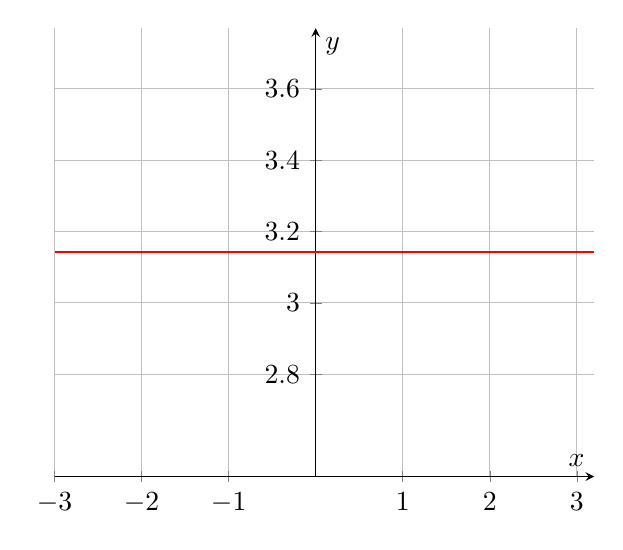
\begin{tikzpicture}
			\begin{axis}[
					xlabel={$x$},
					ylabel={$y$},
					domain=-3:3.2,
					samples=100,
					axis lines=middle,
					grid
				]
				\addplot[red,thick]{pi};
			\end{axis}
		\end{tikzpicture}


	\end{center}
}
\problem{
A tarifa de táxi comum em São Paulo, em outubro de 2023, foi definida da seguinte forma: R\$ 6,00 de bandeirada (custo fixo) mais R\$ 4,25 por km rodado (custo variável). Qual é a fórmula ou regra que descreve essa situação? Apresente o gráfico dessa situação. Determine o valor a ser pago (custo total) por uma corrida relativa a um percurso de 5 km.
}
\end{document}
